\documentclass[11pt]{article}
\usepackage[margin=1in]{geometry}
\usepackage{graphicx}
\usepackage{amsmath}
\usepackage{hyperref}
\usepackage{listings}
\usepackage{xcolor}

\definecolor{lightgray}{gray}{0.95}
\lstset{
    backgroundcolor=\color{lightgray},
    basicstyle=\ttfamily\footnotesize,
    frame=single,
    breaklines=true,
    postbreak=\mbox{\textcolor{red}{$\hookrightarrow$}\space}
}

\title{\textbf{Deepfake Video Detection using Vision Transformers}}
\author{Shubh Khandelwal}
\date{CS22B1090}

\begin{document}

\maketitle

\section{Introduction}
This project implements a Vision Transformer-based model to detect fake videos in the Celeb-DF dataset.
This report details the development and evaluation of this project for classifying deepfake videos using a Vision Transformer (ViT) architecture.
The Celeb-DF v2 dataset is used for training and testing the model.
Key evaluation metrics such as Accuracy, AUC, Precision, and Equal Error Rate (EER) are reported.

\section{Requirements}
\begin{lstlisting}
torch
torchvision
scikit-learn
numpy
opencv-python
pandas
\end{lstlisting}

\section{Dataset}
\begin{itemize}
    \item \textbf{Dataset:} Celeb-DF v2
    \item \textbf{Classes:} Real (0) and Fake (1)
    \item \textbf{Total Videos:} Approximately 5639
    \item \textbf{Format:} MP4
\end{itemize}

\section{Preprocessing}
\begin{itemize}
    \item Created custom dataset and dataloader for loading videos from Celeb-DF dataset
    \item Converted video frames from BGR to RGB
    \item Applied resizing and normalization using ImageNet statistics
    \item Selected a fixed number of maximum frames per video (e.g., 32)
    \item Used padding (repeating the last frame) if a video had fewer frames
\end{itemize}

\section{Vision Transformer (ViT) Architecture}
\begin{itemize}
    \item Patch embedding of video frames with embed dimension 768
    \item Implementation of multi head self attention
    \item MLP classification head
    \item Transformer encoder blocks with variable depth to increase or decrease complexity
    \item Use of patch embedding and transformer encoder blocks along with normalization layer and head
\end{itemize}

\begin{figure}[h!]
    \centering
    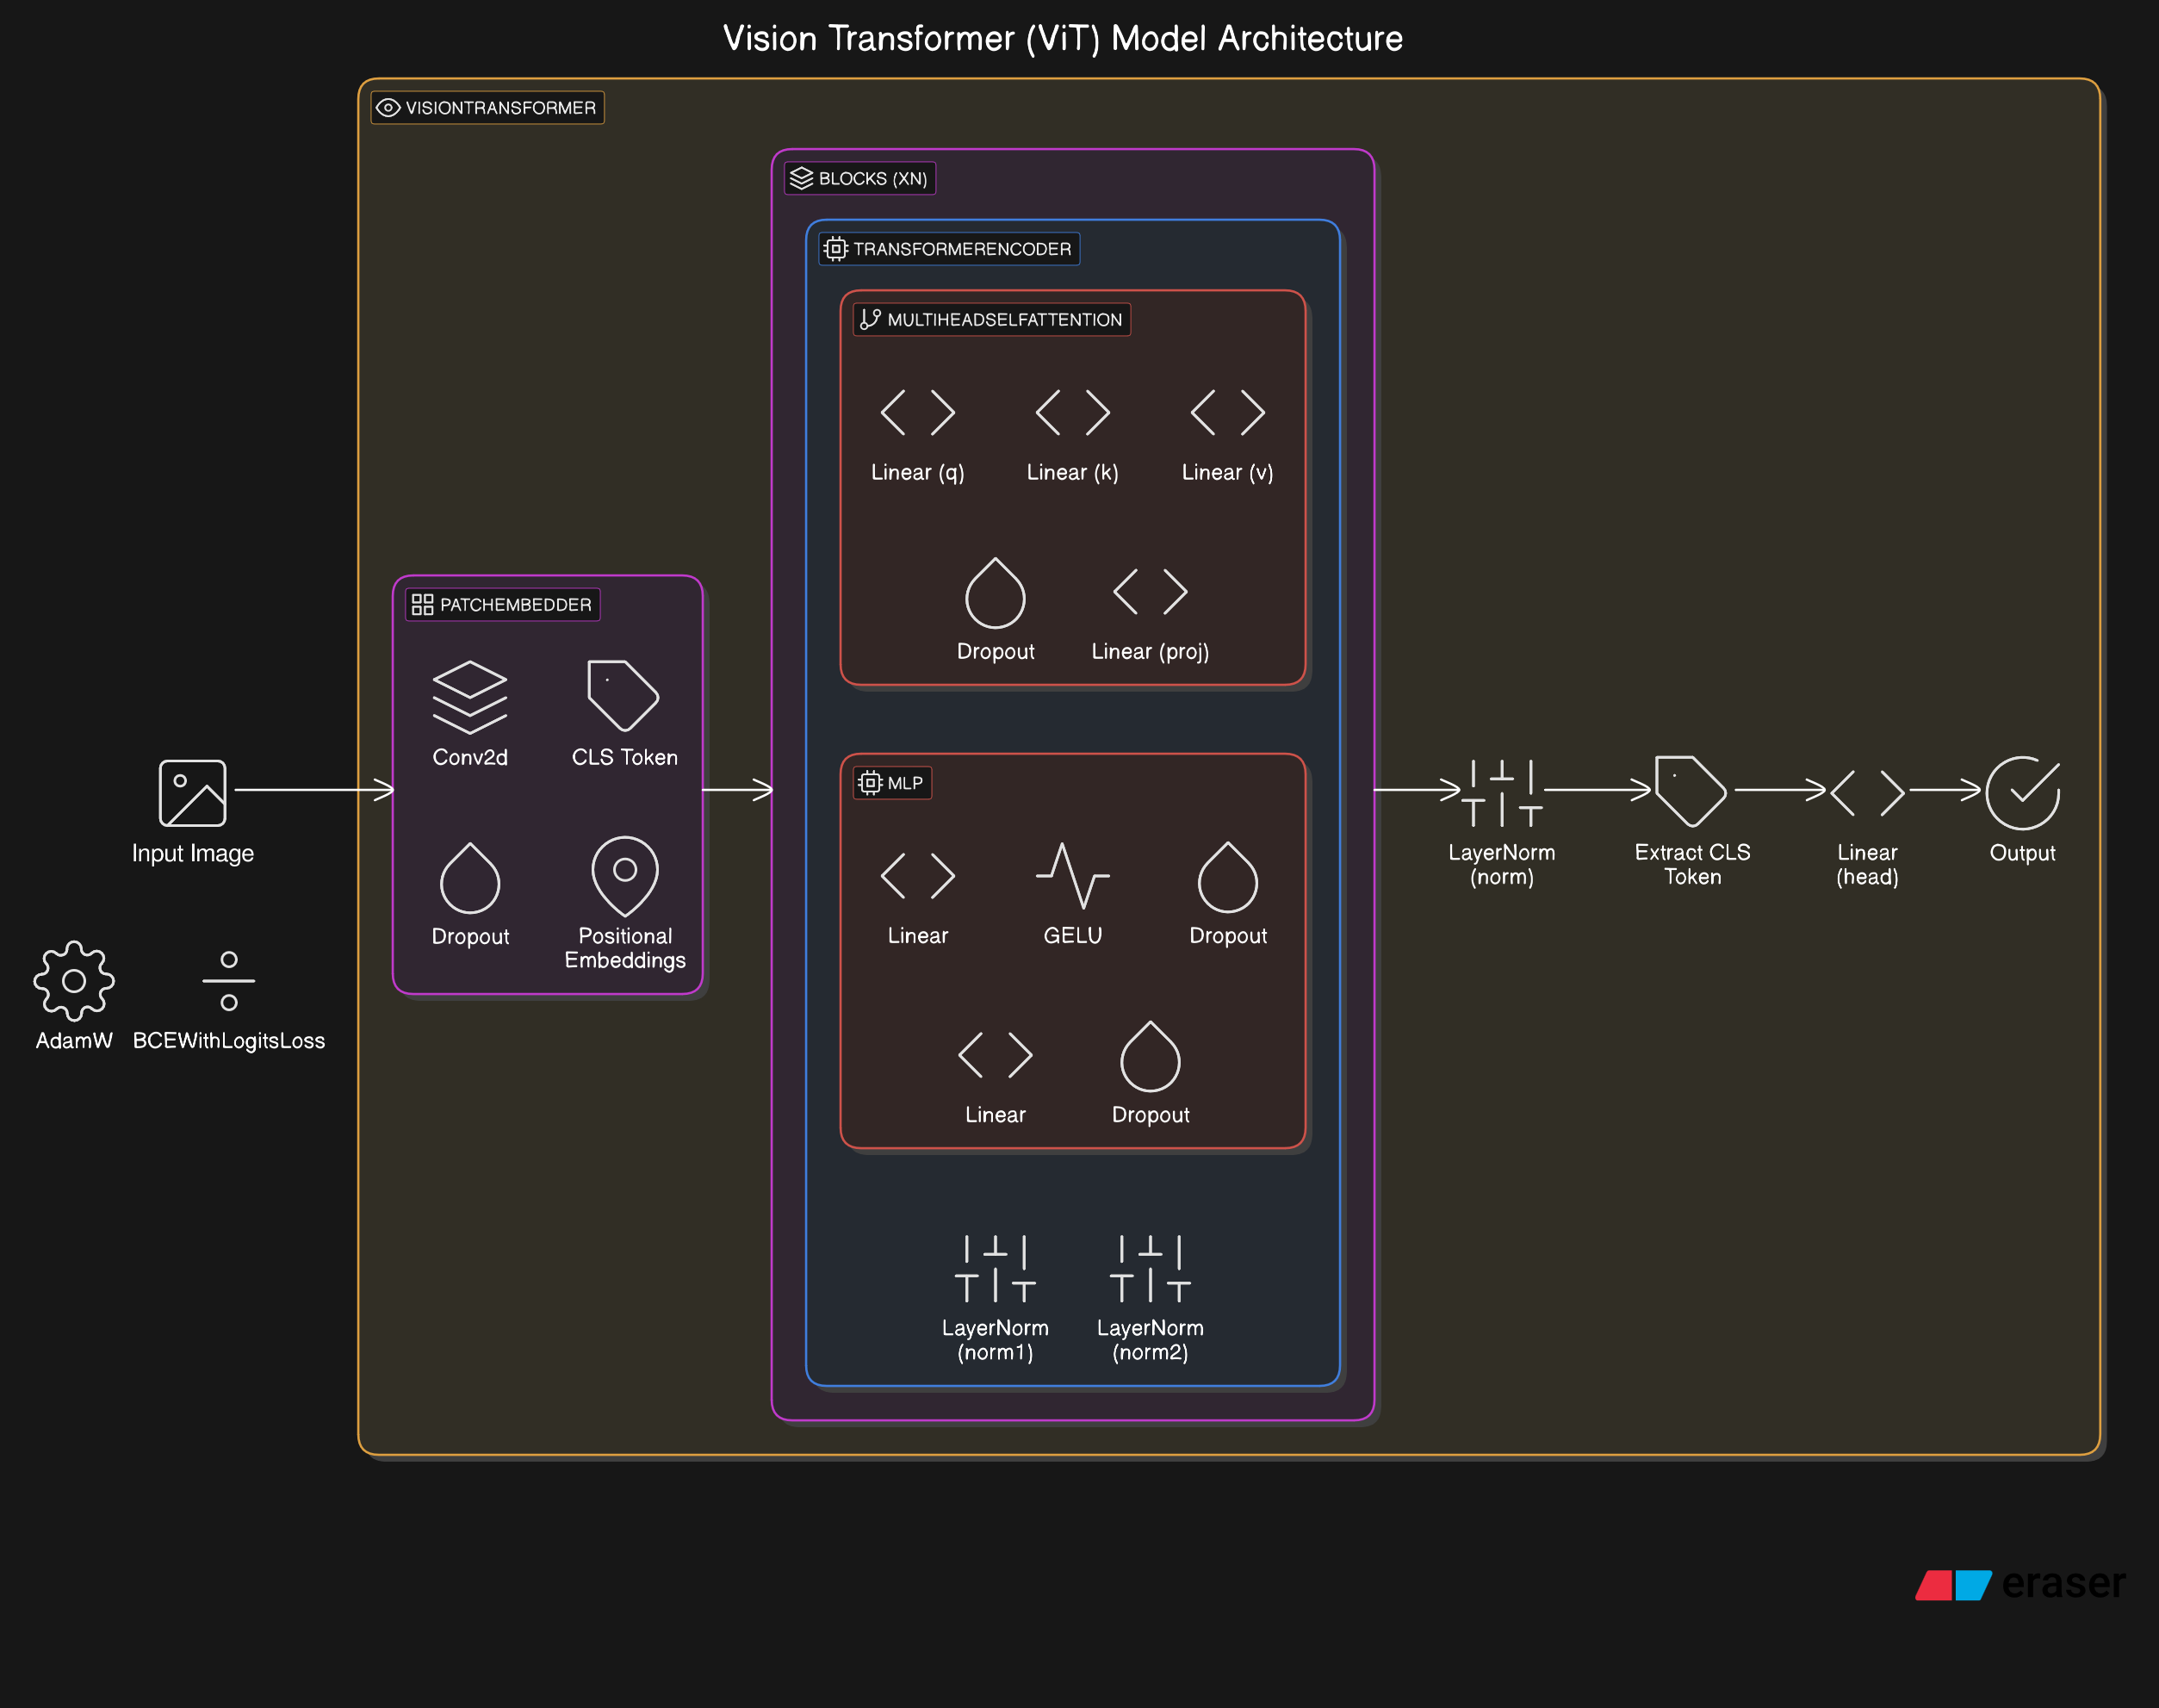
\includegraphics[width=0.9\linewidth]{architecture.png}
    \caption{Block diagram of the Vision Transformer architecture}
    \label{fig:transformer_diagram}
\end{figure}

\pagebreak

\section{Training Details}
\begin{itemize}
    \item Optimizer: AdamW
    \item Learning Rate: 3e-4
    \item Weight Decay: 0.05
    \item Loss Function: BCEWithLogitsLoss
    \item Epochs: 10
    \item Batch Size: 2
\end{itemize}

\section{Evaluation Metrics}
Per-video evaluation using:
\begin{itemize}
    \item Accuracy: 88.52\%
    \item Area Under Curve (AUC): 49.87
    \item Precision: 88.52\%
    \item Equal Error Rate (EER): 0.00
\end{itemize}

\section{References}
\begin{enumerate}
  \item Dosovitskiy, A., Beyer, L., Kolesnikov, A., Weissenborn, D., Zhai, X., Unterthiner, T., ... \& Houlsby, N. (2020). \textit{An image is worth 16x16 words: Transformers for image recognition at scale}. arXiv preprint arXiv:2010.11929.
  \item Tolosana, R., Vera-Rodriguez, R., Fierrez, J., Morales, A., \& Ortega-Garcia, J. (2020). \textit{Deepfakes and beyond: A survey of face manipulation and fake detection}. Information Fusion, 64, 131-148.
  \item Li, Y., Yang, X., Sun, P., Qi, H., \& Lyu, S. (2020). \textit{Celeb-DF: A Large-scale Challenging Dataset for DeepFake Forensics}. In Proceedings of the IEEE/CVF Conference on Computer Vision and Pattern Recognition (pp. 3207-3216).
  \item Vaswani, A., Shazeer, N., Parmar, N., Uszkoreit, J., Jones, L., Gomez, A. N., ... \& Polosukhin, I. (2017). \textit{Attention is all you need}. Advances in neural information processing systems, 30.
\end{enumerate}

\end{document}